% vim: set tw=78 aw:
\documentclass{beamer}

\usepackage[utf8x]{inputenc} % diacritice
\usepackage[romanian]{babel}
\usepackage{hyperref}        % folositi \url{http://...}
% sau \href{http://...}{Nume Link}
\mode<presentation>
\usetheme{CDL}

% Titlul nu foloseşte Unicode pentru că e o problemă căreia nu i-am dat de
% cap.
\title{Cursul de Dezvoltare Liberă}
\subtitle{CDL - Cursul 1}
\institute[ROSEdu]{ROSEdu}
\vskip30pt
\author[Victor]{Victor Cărbune \and \hskip30pt Laura Vasilescu \\ 
  {\small victor@rosedu.org \and \hskip30pt laura@rosedu.org }}

\begin{document}

% Slide-urile cu mai multe părţi sunt marcate cu textul (cont.)
\setbeamertemplate{frametitle continuation}[from second]
% Arătăm numărul frame-ului
\setbeamertemplate{footline}[frame number]

\frame{\titlepage}

\begin{frame}
\tableofcontents
\end{frame}

% NB: Secţiunile nu sunt marcate vizual, ci doar apar în cuprins.
\section{Structura}

% Pentru reamintirea periodică a cuprinsului şi unde ne aflăm:
% \frame{\tableofcontents[currentsection]} - nu mai sunt utile în template-ul
% nou

% Titlul unui frame se specifică fie în acolade, imediat după \begin{frame},
% fie folosind \frametitle
\begin{frame}{Componente}
  \begin{itemize} % Just like normal LaTeX
  \pause
  \item Cursul constă în 8 - 9 întâlniri săptămânale
  \pause
  \vskip17pt
  \item Prezentări ale echipei ROSEdu însoțite de exerciții pragmatice în cadrul laboratorului
  \pause
  \vskip17pt
  \item Contribuții semnificative în cadrul unui proiect Open Source existent
  \pause
  \vskip17pt
  \item Prezentări ale unor invitați din industria IT
  \end{itemize}
\end{frame}

\section{Obiective}

\begin{frame}{Ce își propune cursul?}
  \begin{figure}
    
\includegraphics[scale=0.3]{img/open_source_world.jpg}
  \end{figure}

  \begin{itemize} % Just like normal LaTeX
  \item Să vă familiarizeze cu lumea open source, punându-vă la dispoziție toate resursele necesare
  \end{itemize}
\end{frame}

\begin{frame}{Ce își propune cursul?}
  \begin{figure}
    
\includegraphics[scale=0.4]{img/community.jpg}
  \end{figure}

  \begin{itemize}
  \item Să scurteze drumul implicării voastre într-o comunitate
  \end{itemize}
\end{frame}

\begin{frame}{Ce își propune cursul?}
  \begin{figure}
    
\includegraphics[scale=0.3]{img/motivation.png}
  \end{figure}

  \begin{itemize}
  \item Prim imbold pentru a începe să scrieți cod în cadrul unui proiect Open
  Source
  \end{itemize}
\end{frame}

\begin{frame}{Cum ne propunem să realizăm aceste obiective?}
  \begin{figure}
    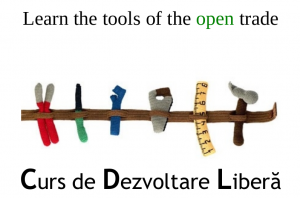
\includegraphics[scale=0.4]{img/open_trade.png}
  \end{figure}

  \begin{itemize} % Just like normal LaTeX
  \pause
  \item Prin prezentarea uneltelor de bază
  \pause
  \item Îndrumându-vă, din punct de vedere tehnic, în realizarea
  contribuțiilor
  \pause
  \item Asigurându-vă un feedback constructiv pe întreaga durată cursului
  (midterm, final reports)
  \end{itemize}
\end{frame}

\section{Motivație}

\begin{frame}{Motivație}
  \begin{itemize} % Just like normal LaTeX
  \pause
  \vskip17pt
  \item Impresionați, realizați primul commit cât mai curând
  \pause
  \vskip17pt
  \item Scrieți despre contribuțiile voastre!
  \pause
  \vskip17pt
  \item Creați-vă o imagine, din punct de vedere tehnic
  \pause
  \vskip17pt
  \item Fiți la actualitate cu ceea ce se întâmplă în domeniul vostru de
  interes
  \pause
  \vskip17pt
  \item Nu în ultimul rând, aveți o întreagă echipă pregătită să vă ajute!
  \pause
  \end{itemize}
\end{frame}

\end{document}
